\documentclass[a4paper,12pt]{article}
\usepackage[a4paper, total={180mm, 272mm}]{geometry}

\usepackage{fontspec}
\setmainfont[Path=fonts/, Extension=.ttf]{ipaexm}

\setlength\parindent{3.5em}
\setlength\parskip{0em}
\renewcommand{\baselinestretch}{1.247}

\usepackage{epic}
\usepackage{eepic}
\usepackage{xcolor}

\usepackage{graphicx}
\graphicspath{{images/}}

\begin{document}

\thispagestyle{empty}

\Large
\noindent \\
Motion Wind Ino\medskip
\par
\normalsize
Allow to add wind flow lines to the image.
\par
It uses an art drawing method, usually seen in animation, to represent a fast motion.\par
Adds the effect of fast motion to the brightest pixels of the image.\\
\\
-{-}- \ Inputs \ -{-}-\\
Source\par
Connect the image to be processed.\\
\\
Reference\par
Connect the reference image to assign the strength of the effect into each pixel.\\
\\
-{-}- \ Settings \ -{-}-\\
Direction\par
Specify the direction of the motion lines.\par
Options available are: Right, Up, Left, Down.\par
The default setting is Right.\par
Direction is fixed for the default orientation of the image. If the column/layer is\par 
rotated, motion lines will rotate with it.\\
\\
Dark\par
When inactive motion lines will spread from brightest parts of the image.\par
When active motion lines will spread from darkest parts of the image..\par
The default setting is inactive.\\
\\
Alpha Rendering\par
This option is valid only when there is an Alpha channel.\par
When inactive, it masks the changes in the RGB values using the original Alpha\par 
of the image.\par
When active, the effect will be able to modify the Alpha channel, extending it\par 
as necessary to reproduce the full span of the effect.\par
The default setting is ON.\\
\\
Length Min\\
Length Max\par
Specify the length of the motion lines.\par
The unit is millimeters.\par
Specify a value in the range from 0 to 1000.\par
Decimal places are also taken into account, for subtle changes in the length.\par
If Min and Max are different, the length of each motion line will be random, between\par 
those values.

\newpage

\thispagestyle{empty}

\ \vspace{-0.2em}
\par
When Min and Max are the same, all motion lines will have the same length.\par
The default value for Min is 0, and Max is 8.573.\par
-{-}> See \textquotedbl Figure 1:\ \ Length Wind\textquotedbl \ .\par
-{-}> See \textquotedbl Figure 4:\ \ Force is 1 and Density is 1\textquotedbl \ .\par
-{-}> See \textquotedbl Figure 7:\ \ Length Wind and Force is 10\textquotedbl \ .\\
\\
Length Bias\par
Allows to introduce a deviation in the random pattern of the length.\par
Using values between 0.1 and 1.0, will make prevail shorter lines.\par
Using a value of 1.0, the pattern will be uniform.\par
Using values between 1.0 and 10.0, will make prevail longer lines.\par
The default value is 1.\par
-{-}> See \textquotedbl Figure 1:\ \ Length Wind\textquotedbl \ .\\
\\
Length Seed\par
This seed controls the random pattern for the length.\par
Specify an integer value greater than or equal to 0.\par
If the same value is given to the same image, it will produce the same pattern.\par
Changing the value will produce different patterns.\par
For example, if you want an ever changing pattern of lines from a single image,\par
you can animate the seed value on a frame by frame basis.\par
The default value is set to 1.\\
\\
Force Min\\
Force Max\par
Allows to define the decay rate of the motion lines.\par
Values between 0.1 and 1.0, will cause a fast decay rate,\par
A value of 1.0 will produce a linear decay rate,\par
Values between 1.0 and 10.0, will cause a slow decay rate,\par
If Min and Max are different, the decay rate of each motion line will be random,\par 
between those values.\par
When Min and Max are the same, all motion lines will have the same decay rate.\par
The default value is 1 for both.\par
-{-}> See \textquotedbl Figure 2:\ \ Force Wind\textquotedbl \ .\par
-{-}> See \textquotedbl Figure 5:\ \ Force is 0.1\textquotedbl \ .\par
-{-}> See \textquotedbl Figure 7:\ \ Length Wind and Force is 10\textquotedbl \ .\\
\newpage

\thispagestyle{empty}

\ \vspace{-0.2em}
\\
Force Bias\par
Allows to introduce a deviation in the random pattern of decay.\par
Using values between 0.1 and 1.0, will make a strong decay prevail.\par
Using a value of 1.0, the decay pattern will be uniform.\par
Using values between 1.0 and 10.0, will make a weak decay prevail.\par
The default value is 1.\par
-{-}> See \textquotedbl Figure 2:\ \ Force Wind\textquotedbl \ .\\
\\
Force Seed\par
This seed controls the random pattern for the decay rate.\par
The options are similar to \textquotedbl Length Seed\textquotedbl .\\
\\
Density Min\\
Density Max\par
Allows to define the density of the motion lines.\par
If it is 0, there will be no motion lines effect.\par
Values between 0 and 1.0 will produce low densities.\par
A value of 1.0 will produce a standard density.\par
Values greater than 1.0 will produce high densities. The maximum value is 100.\par
If Min and Max are different, density will be random between those values.\par 
When Min and Max are the same, density will be uniform.\par 
The default value is 1 for both.\par
-{-}> See \textquotedbl Figure 3:\ \ Density Wind\textquotedbl \ .\par
-{-}> See \textquotedbl Figure 6:\ \ Density is 0.2\textquotedbl \ .\\
\\
Density Bias\par
Allows to introduce a deviation in the random pattern of density.\par
Using values between 0.1 and 1.0, will make lower densities prevail.\par
Using a value of 1.0, the density pattern will be uniform.\par
Using values between 1.0 and 10.0, will make higher densities prevail..\par
The default value is 1.\par
-{-}> See \textquotedbl Figure 3:\ \ Density Wind\textquotedbl \ .\\
\\
Density Seed\par
This seed controls the random pattern for the density.\par
The options are similar to \textquotedbl Length Seed\textquotedbl .\\

\newpage

\thispagestyle{empty}

\ \vspace{-0.2em}
\\
In order to achieve a uniform lines effect:\par
The same values should be assigned to \textquotedbl Length Min\textquotedbl \ and \textquotedbl Length Max\textquotedbl ,\par
\textquotedbl Force Min\textquotedbl \ and \textquotedbl Force Max\textquotedbl ,
\textquotedbl Density Min\textquotedbl \ and \textquotedbl Density Max\textquotedbl \ parameters,\par 
to produce uniform lines.\\
\\
To synchronize random patterns:\par
If \textquotedbl Length Seed\textquotedbl , \textquotedbl Force Seed\textquotedbl , and \textquotedbl Density Seed\textquotedbl \ are set to the same value\par 
at the same frame, its patterns will match, and it will become stronger and\par 
weaker at the same time.\par
Using different values will produce different patterns for each parameter.\\
\\
To fix a random pattern when the camera is moving:\par
When moving the camera over a background image, the random pattern changes\par 
on each frame according to the change of the picture.\par
To fix the pattern the entire background image must be processed.\\
-{-}-{-}-{-}\\
\\
Length Ref\par
When inactive there will be no reference image driving the Length.\par
When active, the image connected to the Reference port will drive the Length.\par
The values of the selected channel in the Reference parameter, will drive the Length.\par
If no reference image is available, the length will be determined by the Source image\par 
brightness.\par
The darker the pixel where lines begin, the shorter they will be.\par
As the whole image tone is lowered, please adjust the Min and Max Length values.\par
The default state is inactive.\\
\\
Force Ref\par
When inactive there will be no reference image driving the Force.\par
When active, the image connected to the Reference port will drive the Force.\par
The values of the selected channel in the Reference parameter, will drive the Force.\par
If no reference image is available, the force will be determined by the Source image\par 
brightness.\par
The darker the pixel where lines begin, the weaker they will be.\par
As the whole image tone is lowered, please adjust the Min and Max Force values.\par
The default state is inactive.\\
\newpage

\thispagestyle{empty}

\ \vspace{1.3em}
\\
Density Ref\par
When inactive there will be no reference image driving the Density.\par
When active, the image connected to the Reference port will drive the Density.\par
The values of the selected channel in the Reference parameter, will drive the\par 
Density.\par
If no reference image is available, the density will be determined by the Source\par 
image brightness.\par
The darker the pixel where lines begin, the thinner they will be.\par
As the whole image tone is lowered, please adjust the Min and Max Density values.\par
The default state is inactive.\\
\\
Reference\par
Choose how the Reference image values are used to set the strength of the effect\par 
into each pixel.\par
Choose from Red/Green/Blue/Alpha/Luminance.\par
Choose Nothing to disable the effect.\par
The default value is Red.

\newpage

\thispagestyle{empty}

\ \vspace{-0.2em}
\par
\noindent Figure 1:\ \ Length Wind

\large
\noindent \begin{picture}(0,0)
\linethickness{0.01em}
\put(1,-198.5){\line(1,0){198}}
\put(9,-200.5){\line(0,1){62}}
\drawline[0](9,-143)(193,-198.5)
\drawline[0](9,-143)(102,-198.5)
\drawline[0](9,-143)(28,-198.5)
\put(0.5,-135){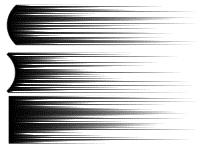
\includegraphics[width=13.9em]{MotionWindInoFunction1LengthWindA}}
\put(142,-171.5){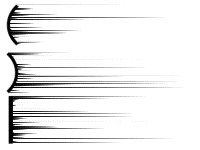
\includegraphics[width=13.9em]{MotionWindInoFunction1LengthWindB}}
\put(284.5,-200){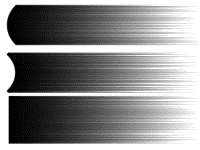
\includegraphics[width=13.9em]{MotionWindInoFunction1LengthWindC}}
\put(209,-16.5){\normalsize{Bias is 0.1}}
\put(351,-45){\normalsize{Bias is 10}}
\end{picture}\\[12.6em]

\normalsize
\noindent Figure 2:\ \ Force Wind

\large
\noindent \begin{picture}(0,0)
\linethickness{0.01em}
\put(1,-198.5){\line(1,0){198}}
\put(9,-200.5){\line(0,1){62}}
\drawline[0](9,-143)(193,-198.5)
\spline(9,-143)(129,-150)(188,-180)(195,-198.5)
\spline(9,-143)(20,-168.5)(85,-192.5)(193,-198.5)

\put(0.5,-135){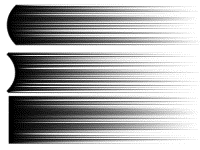
\includegraphics[width=13.9em]{MotionWindInoFunction2MotionWindA}}
\put(142,-171.5){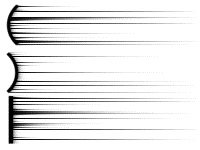
\includegraphics[width=13.9em]{MotionWindInoFunction2MotionWindB}}
\put(284.5,-200){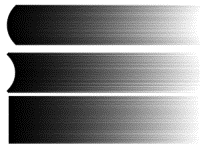
\includegraphics[width=13.9em]{MotionWindInoFunction2MotionWindC}}
\put(209,-16.5){\normalsize{Bias is 0.1}}
\put(351,-45){\normalsize{Bias is 10}}
\end{picture}\\[12.65em]

\normalsize
\noindent Figure 3:\ \ Density Wind

\large
\noindent \begin{picture}(0,0)
\linethickness{0.01em}
\put(1,-198.5){\line(1,0){198}}
\put(9,-200.5){\line(0,1){62}}
\drawline[0](9,-143)(193,-198.5)
\drawline[0](9,-166.5)(193,-198.5)
\drawline[0](9,-192)(193,-198.5)

\put(0.5,-135){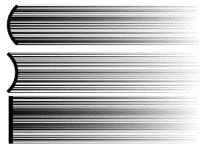
\includegraphics[width=13.9em]{MotionWindInoFunction3DensityWindA}}
\put(142,-171.5){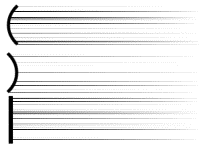
\includegraphics[width=13.9em]{MotionWindInoFunction3DensityWindB}}
\put(284.5,-200){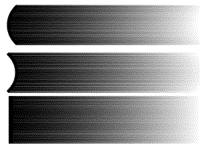
\includegraphics[width=13.9em]{MotionWindInoFunction3DensityWindC}}
\put(209,-16.5){\normalsize{Bias is 0.1}}
\put(351,-45){\normalsize{Bias is 10}}
\end{picture}

\newpage

\thispagestyle{empty}

\ \vspace{-0.1em}
\par
\large
\noindent \hskip 10.5em Length Min equal Max Wind\\[-0.15em]
\normalsize
Figure 4:\ \ Force is 1 and Density is 1

\large
\noindent \begin{picture}(0,0)
\put(28.5,-132){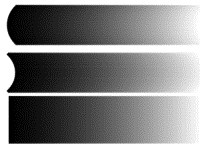
\includegraphics[width=13.9em]{MotionWindInoFunction4}}
\end{picture}\\[7.6em]

\large
\noindent \hskip 10.5em Length Min equal Max Wind\\[-0.15em]
\normalsize
Figure 5:\ \ Force is 0.1

\large
\noindent \begin{picture}(0,0)
\put(28.5,-132){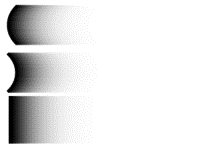
\includegraphics[width=13.9em]{MotionWindInoFunction5}}
\end{picture}\\[7.6em]

\large
\noindent \hskip 10.5em Length Min equal Max Wind\\[-0.15em]
\normalsize
Figure 6:\ \ Density is 0.2

\large
\noindent \begin{picture}(0,0)
\put(28.5,-132){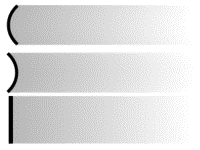
\includegraphics[width=13.9em]{MotionWindInoFunction6}}
\end{picture}\\[7.4em]

\normalsize
\noindent Figure 7:\ \ Length Wind and Force is 10

\large
\noindent \begin{picture}(0,0)
\put(28.5,-132){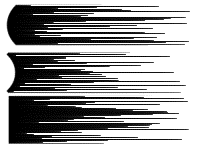
\includegraphics[width=13.9em]{MotionWindInoFunction7}}
\end{picture}

\end{document}